\subsection{Discussion}
In this section, we discuss the deficiencies of our approach, analyse their causes and propose some possible improvements.

\subsubsection{Deficiency of 2D Coordinate Labelling}
\label{2d_def}
\paragraph{Deficiency of Our Labelling Approach}
Our approach requires accurate 2D characteristic points to perform 2D-3D matching to calculate the location and orientation of the vehicles. However precisely labelling these points is demanding or even impossible for some vehicles with our semi-automatic labelling tool. The deficiency of labelling results from our labelling approach and the KITTI dataset.

Due to the variety of dimensions and shapes of vehicles, it is very hard to find a model that exactly matches the target vehicle with a small set of models. But if we expand the model set to cover all vehicles, the required quantity is too huge to satisfy. Therefore, we can only use a small set of models which means that the approximation and scaling are inevitable. And this will introduce errors to the labelling of 2D coordinates. Figure \ref{figure:label_def} (a) and (b) show two bad labelled examples. The imprecision of (a) results from the approximation of model matching, \ie most points are labelled correctly but point 1-6 are not. This is because the model can't perfectly fit the vehicle. The wrongly labelled points around wheels roots in the scaling the model to fit the vehicle so that, for example, the distance between point 4 and 8 are larger than the diameter of the wheel. The other pairs of points around the wheel have similar situation so that most points are not labelled correctly for this vehicle.

\begin{figure}[H]		
	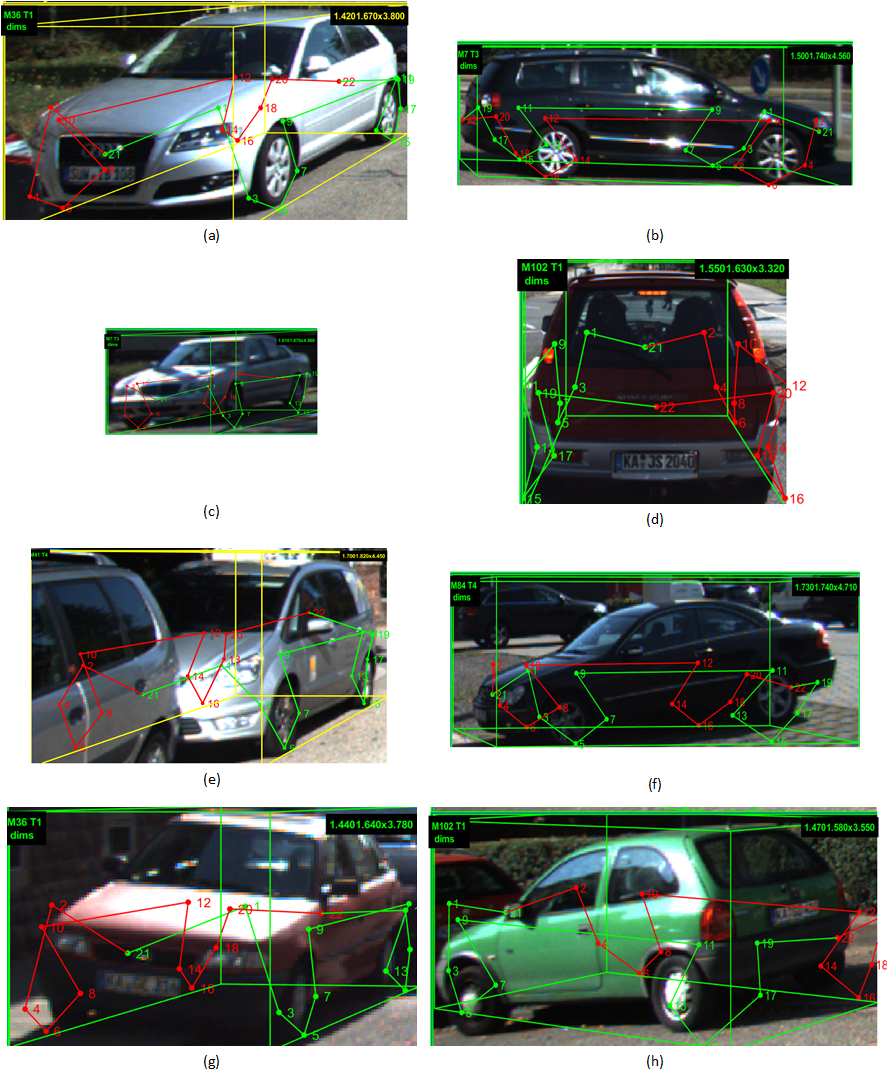
\includegraphics[width=0.8\textwidth]{label_def.png}
	\caption{Labelling examples for 2D points with original size. (a). Approximation results in inaccurate label for point 1-6. (b). Scaling change the relative distance between points which lead to bad labelling for points around the wheels. (c). One of the very small vehicles in image is able to be labelled with our approach. (d). The example that the side faces are not visible is able to be labelled with our approach. (e). The occluded vehicle can also be labelled with our approach. (f). The 3D bounding box ground truth of this vehicle is not correctly labelled in KITTI dataset. (g). KITTI doesn't consider the rotation along the roll axis, which results in bad labelling. (h). KITTI doesn't consider the rotation along the pitch axis, which results in totally wrong labelling.}
	\centering
	\label{figure:label_def}
\end{figure}

\paragraph{Deficiency of KITTI Dataset Labelling}
Our labelling approach requires very accurate label of the dataset because 2D points are very sensitive to the exact location of the target vehicle. But some of the KITTI images are not labelled so well that our approach makes mistakes. There are three main deficiencies of the KITTI labelling as shown in Figure \ref{figure:label_def} (f), (g), and (h). (f) shows the 3D bounding box ground truth of this vehicle is not correctly labelled. The 3D bounding box doesn't encompass the vehicle, especially the rear part, which leads to wrong labelling. (g) and (h) shows that our approach wrong labels the 2D points due to the assumption of KITTI that the vehicle only rotate along the yaw axis rather than the roll and pitch axis.


\paragraph{Possible Improvements}
Despite the drawbacks of our labelling approach, it has still has some advantages. Our approach can label very small vehicles in the image as shown in Figure \ref{figure:label_def} (c). Besides, it can label the self-occluded points as in Figure \ref{figure:label_def} (d) and the occluded and truncated points in Figure \ref{figure:label_def} (e). 

Therefore, if labelling labour is allowed, we can manually label the visible points for big vehicles and use the projection property and the geometry constraints to automatically generate the corresponding points. Therefore we have more accurate points for big vehicles. And for small and highly occluded or truncated vehicles, it is suitable to use our approach to label them. Because manually labelling these special vehicles is almost impossible and the error of our labelling approach can be decreased due to the quantities.


\subsubsection{Deficiency of Visibility Labelling}
\paragraph{Deficiency of Our Labelling Approach}
As described in Section \ref{visibility}, we label the visibility property of characteristic points with the help of the rotation $r_y$, other labelled objects, and the size of images. But there are two main shortcomings. The first one is that the 2D bounding box of a vehicle is larger in image than its real shape which makes our approach mistake the visible or self-occlude points as occluded. Figure \ref{figure:visib_def} (a). shows an example of labelling the self-occluded points as occluded, which leads to wrong labels. Another shortcoming is that our approach can't take the unlabelled objects into consideration so that it automatically ignores than during labelling. Figure \ref{figure:visib_def} (b) and (c) show two examples for this case. Our approach can't consider the traffic sign in (b) and the building in (c) and thus, it fails to label these occluded points correctly.

\begin{figure}[H]		
	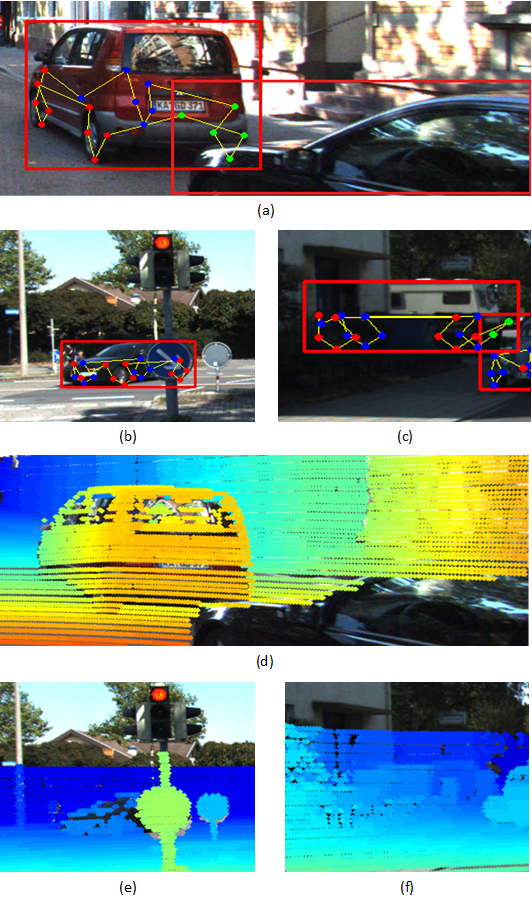
\includegraphics[width=0.7\textwidth]{visib_def.png}
	\caption{Labelling examples for visibility with original size. (a). The 2D bounding box is larger than the vehicle's real size, which results in labelling the self-occluded points as occluded. (b). KITTI doesn't label the traffic sign so that our approach can't label the occluded points correctly. (c). KITTI doesn't label the building so that our approach can't label the occluded points correctly.}
	\centering
	\label{figure:visib_def}
\end{figure}

\paragraph{Possible Improvements}

KITTI offers the LiDAR data for all images, which can provide the depth information of each pixel point in image or at least of a very small region. And based on the ground truth of location, orientation, and dimension of vehicles given by KITTI, we can calculate the depth of points distributed on the surface of the vehicles. By comparing these two kinds of depth information, we can correctly figure out whether there is some object in front of the target vehicle or not and which parts of the target vehicle are occluded, and thus we can classify the visibility properties correctly. Figure \ref{figure:visib_def_lidar} shows the images with LiDAR projection for examples in Figure \ref{figure:visib_def}. With the LiDAR depth information, we can easily classify the points around rear in (a) as self-occluded, and the occluded objects in (b) and (c) can be clearly detected and thus, we can assign the points whose depth is deeper than these objects as occluded. Therefore, for more accurate visibility labelling, it is worth making use of the LiDAR data.

\begin{figure}[H]		
	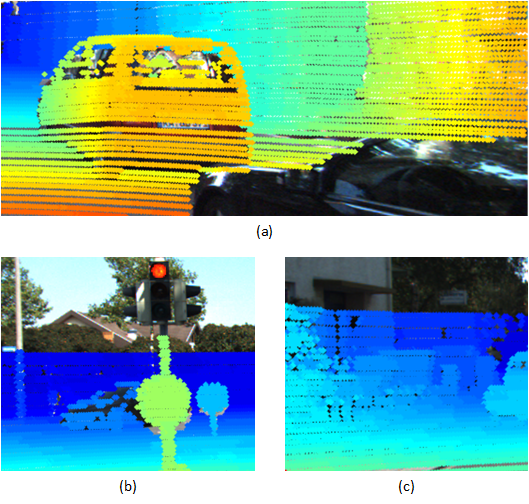
\includegraphics[width=0.7\textwidth]{visib_def_lidar.png}
	\caption{Images with LiDAR data projection for examples in Figure \ref{figure:visib_def} (a), (b), and (c) respectively.}
	\centering
	\label{figure:visib_def_lidar}
\end{figure}

\subsubsection{Deficiency of Template Matching}
In our approach, there are two situations where template matching is performed to fit a target vehicle with a 3D vehicle model. The first one is during labelling, when a 3D vehicle sketch is required to be projected into the KITTI images to generate 2D coordinates of key points for a target vehicle. And the model is selected via dimension matching. Another is during inference phase, where one 3D sketch is needed to generate the corresponding 3D coordinates of the key points for the target vehicle in the world coordinate system. The time the model is selected based on the estimated template proximity vector, \ie the ratios of 3 dimensions between the target vehicle and all 3D vehicle models.

For both cases, the most fundamental drawback is that we can only match the target vehicle with an approximate model based on the Dims strategy. This would results in errors in 2D and 3D coordinates of key points and thus impacts the final 3D vehicle pose estimation.

\paragraph{Possible Improvements}
As we mentioned before, the geometric property of 3D sketch relies heavily on the type of the vehicles. Therefore, a possible improvement for matching is to introduce type information into the matching phase. And there are some out-off-shelf frameworks can provide this kind of information \cite{DBLP:journals/corr/YangLLT15, 7780697, 7410527, DBLP:journals/corr/DehghanMSO17}, \ie Afshin \etal provide a network can recognize the Make and Model of vehicles \cite{DBLP:journals/corr/DehghanMSO17}. 

In sum, the optimal matching strategy is we first collect a 3D vehicle dataset where the distribution of vehicle dimensions covers the main part of the distribution of real vehicle dimensions in a fine-grained style, and during the matching, we first estimate the type of the vehicle and then select the best model via dimension matching from the same category. 

\subsubsection{Deficiency of Whole Approach}
The first unpleasant thing of this approach is the additional labelling work. This is so time consuming that it takes more than two month to find a proper method to generate the additional labels at an acceptable accuracy level. Besides, even with this method, the accuracy of the labels is compromised.

Moreover, our approach requires an additional 3D vehicle model dataset to encode the geometry information of vehicles, which makes it hard to generalize to vehicles without a corresponding model in the model dataset. For example, our approach can't perform accurate 3D pose estimation of buses because we don't include the bus models.

According to the competition results of KITTI 3D object detection, the approach that relies on single sensor can't compare with those making use of multi-sensor data \cite{3dobject}. RGB images captured by cameras have high resolution and good texture knowledge but lack depth information, which cloud points collected by LiDAR have 3D information of the scene but the resolution is relative lower and lack texture information. Therefore we think the best performance would be achieved by some approach driven by sensor fusion. If we have can start this task again, this is the first direction we will explore.





